\documentclass{article}
\usepackage{iclr2026_conference,times}

\usepackage{hyperref}
\usepackage{url}
\usepackage{amsmath,amssymb,amsfonts}
\usepackage{booktabs}
\usepackage{graphicx}
\usepackage[table]{xcolor}
\usepackage{multirow}
\usepackage{enumitem}
\usepackage{amsthm}
\usepackage{microtype}
\usepackage{array}
\usepackage{float}
\usepackage{tikz}
\usetikzlibrary{arrows.meta}

\hypersetup{
  colorlinks=true,
  citecolor=teal!70!black,
  linkcolor=teal!70!black,
  urlcolor=teal!70!black,
  hypertexnames=false
}

\newtheorem{proposition}{Proposition}

\newcommand{\tap}{\textsc{ACE}}
\newcommand{\far}{\textsc{FAR-Hammer}}
\newcommand{\fars}{\textsc{FAR}}
\newcommand{\best}[1]{\textbf{\textcolor{teal!70!black}{#1}}}
\newcommand{\gain}[1]{\textcolor{teal!70!black}{#1}}
\newcommand{\warn}[1]{\textcolor{orange!80!black}{#1}}
\newcommand{\metricup}[1]{#1$\uparrow$}
\newcommand{\metricdown}[1]{#1$\downarrow$}
\newcolumntype{L}[1]{>{\raggedright\arraybackslash}p{#1}}

\title{Premise Selection Is Not Enough: Action-Conditional Evidence Allocation for Lean}
\author{Anonymous}

\begin{document}
\maketitle

\begin{abstract}
Premise selection is usually treated as a ranking problem: choose useful lemmas, pass them to a Lean prover, and hope reconstruction succeeds. We argue that this view is missing a \textbf{second intervention}. A selected name must still be compiled into the proof interface that can consume it: Hammer facts, HammerCore inputs, simp lemmas, local elimination facts, Aesop fact rules, or Aesop simp rules. We introduce \tap, a \textbf{typed evidence compiler} for \emph{action-conditional evidence allocation} in Lean. The core finding is counterintuitive but repeatable: once the candidate names are fixed, \textbf{small typed portfolios} can recover nearly all tested oracle headroom, while learned routers do not yet beat the fixed typed control. In a Mathlib 4.30 + LeanHammer 4.30 pre-theorem replay harness, the mixed oracle-core/retrieved action grid solves 58/230 kernel-verified goals versus 38/230 for the best single action; a four-retry fixed portfolio reaches 57/230 out of fold. Removing traced proof-core names still leaves a retrieved-only compiler effect: empty Hammer solves 29/230, the best standalone action solves 35/230, and a fixed portfolio reaches the 52/230 typed oracle. To check that the effect is not only a post-hoc fit to the 230-goal matrix, we freeze the retrieved-only four-action portfolio and evaluate two disjoint fresh folds: on 432 replayable holdout goals, empty Hammer solves 30, the best singleton solves 54, the frozen K=4 portfolio solves 67, and the tested-action oracle is 68. Exact Aesop controls further constrain the mechanism: joint oracle-core plus retrieved exposure is best at 38/230, but identity and simps-only controls reach 36/230 and 35/230, so the supported claim is \textbf{source/interface sensitivity} rather than a large pure facts-versus-simps complementarity. \tap{} is therefore not a new retriever or an adaptive-router victory; it is evidence that premise selection is incomplete until selected names are typed into executable Lean proof actions.
\end{abstract}

\section{Introduction}

Lean hammers and neural theorem provers depend on premise selection: given a proof goal, the system must choose accessible lemmas that make proof search tractable and reconstructable in Lean. Modern systems therefore invest heavily in retrieving better premises before running a backend prover \citep{yang2023leandojo,zhu2025premise,gao2026leansearch}. This framing is necessary but incomplete. A selected Lean name is not yet an executable proof-search intervention; it must be represented for the tactic that will consume it. The same name may be useful as a Hammer fact, inert as a simp lemma, harmful as an Aesop rule, or useful only after being paired with a different interface.

This interface decision is easy to overlook because it is not the same as ordinary tactic selection. We are not only choosing whether to call Hammer, Aesop, or simplification. We are choosing how a fixed source of evidence should enter each proof mechanism: as facts, simp rules, HammerCore inputs, local elimination facts, or multi-channel Aesop programs. Under bounded search, more evidence is also not monotonic. Additional names can improve proof-core coverage while increasing branching, timeouts, or reconstruction ambiguity. Thus a high-recall premise list can still fail if it is compiled into the wrong Lean interface.

We propose \tap, an action-conditional evidence allocator for bounded Lean proof search. Given a replayable theorem context and a candidate set, \tap{} compiles selected names into typed proof actions and checks each action in Lean. Every comparison starts from the same empty-premise Hammer attempt and then spends a fixed retry budget. This protocol turns the main question into a reviewer-checkable intervention study: after names have been proposed, how much verified headroom comes from assigning them to the right proof interface?

The empirical answer is surprisingly strong for simple typed portfolios. In a Mathlib 4.30 + LeanHammer 4.30 pre-theorem replay harness, we identify 230 replayable goals from 490 cleaned traced-corpus goals. A mixed source pool of traced oracle-core names and learned retrieved candidates gives a typed action oracle of 58/230, compared with 38/230 for the best single action. A four-retry fixed typed portfolio after \texttt{hammer\_empty} reaches 57/230 out of fold and 58/230 when fit on all training data. Homogeneous K=4 controls are much weaker: Aesop-only reaches 49/230, HammerCore-only and simplification-only reach 41/230, and Hammer-only reaches 32/230. The effect is therefore typed diversity, not simply more calls to one backend.

We then remove the most obvious source of concern: traced proof-core assistance. In a retrieved-only anchor on the same 230 replayable goals, empty Hammer solves 29/230 and the best standalone action solves 35/230, while a fixed typed portfolio reaches the 52/230 typed oracle out of fold. To test whether this is a post-hoc peculiarity of the 230-goal matrix, we freeze the retrieved-only four-action portfolio and evaluate two fresh disjoint folds with zero overlap against the original goals. Across 432 replayable holdout goals, empty Hammer solves 30, the best singleton solves 54, K=3 and K=4 solve 67, and the tested-action oracle is 68. This does not make \tap{} a full theorem-proving leaderboard system, but it does give prospective evidence that typed compilation survives beyond the matrix used to discover it.

The mechanism is also narrower than our early experiments suggested. Aesop with oracle-core plus retrieved evidence exposed jointly as facts and simp lemmas proves 38/230 goals, compared with 29/230 for empty Aesop. Exact controls show that this is not a large isolated facts-versus-simps complementarity: identity exposure proves 36/230, simps-only proves 35/230, facts-only proves 32/230, retrieved-only joint exposure proves 34/230, and oracle-core-only joint exposure proves 35/230. The robust readout is that selected evidence has source-dependent and interface-dependent behavior; the paper does not need the stronger channel-complementarity claim.

This paper makes three contributions. First, we formulate action-conditional evidence allocation as a distinct layer after premise retrieval: selected names must be typed into Lean proof interfaces, not only ranked. Second, we implement \tap{} in a real Mathlib 4.30 + LeanHammer 4.30 pre-theorem replay harness and show that fixed typed portfolios recover nearly all tested oracle headroom in a mixed-source matrix, a retrieved-only anchor, and frozen fresh-holdout folds. Third, we report the boundaries that keep the claim honest: broad insertion can hurt, strict syntactic filtering does not explain the gains, exact Aesop controls weaken a tempting complementarity story, and logistic/ComplementNB allocators do not yet beat the fixed typed control.

The scope is deliberately narrower than a full theorem-proving leaderboard. The retrieved-only and fresh-holdout experiments test the downstream compiler once candidate names are fixed; they are not official reproductions of LeanSearch v2 or another complete global retrieval system. We also distinguish bridge replay from open-ended proof generation. These boundaries sharpen rather than weaken the claim: premise selection is incomplete until selected evidence is compiled into the Lean interface that can actually use it.

\section{Related Work}

\paragraph{Premise selection and hammers.}
Premise selection is a long-standing interface between theorem provers and large formal libraries. LeanDojo introduced retrieval-augmented theorem proving infrastructure in Lean \citep{yang2023leandojo}; recent Lean-hammer work studies learned premise ranking and ATP integration \citep{zhu2025premise}; and LeanSearch v2 focuses on global Lean 4 premise retrieval \citep{gao2026leansearch}. These systems motivate our setting: a retriever proposes useful names before proof search. \tap{} studies the next decision after retrieval: how those names should be represented for Lean's consuming interface.

\paragraph{Proof-action control and feedback.}
Tactic-selection systems such as TacticToe choose tactics or tactic sequences \citep{gauthier2021tactictoe}, while recent Lean systems use compiler or verifier feedback for proof repair, agentic search, or process supervision \citep{wang2026repairlean,ospanov2025apollo,ma2026oprover,kim2026process,huang2025leanprogress,hu2024minictx}. \tap{} is narrower: it does not edit proof text or propose new theorem-level plans. It fixes a candidate evidence source and tests the typed action by which selected names enter Hammer, HammerCore, simplification, local elimination, and Aesop.

\section{Problem Formulation}

\paragraph{Action-conditional evidence allocation under a fixed retry budget.}
Let $g$ be a Lean goal and let $\mathcal{A}(g)$ be the accessible name set induced by imports, namespaces, declarations, and local context. A typed proof action is a pair $a=(\tau,P)$, where $\tau$ is a Lean interface such as Hammer, HammerCore, simplification, local elimination, or Aesop, and $P\subset \mathcal{A}(g)$ is the set of names exposed through that interface. More generally, a typed evidence program is an assignment
\[
z_{p,\tau}\in\{0,1\}, \qquad \sum_{p\in\mathcal{A}(g)} z_{p,\tau}\le b_\tau,
\]
where $z_{p,\tau}=1$ means that name $p$ is exposed to interface channel $\tau$ under channel budget $b_\tau$. The same name may receive multiple interface labels: an Aesop joint facts+simps action is one compiled program, not two independent retries. A compiler $C(z)$ maps this assignment to Lean tactic syntax, such as Hammer facts, HammerCore inputs, simplifier lemmas, local elimination facts, Aesop safe facts, and Aesop simp rules. This separates four decisions that are often conflated: candidate provenance, channel eligibility, channel assignment, and outer action scheduling.

An evidence allocator chooses a sequence of typed programs,
\[
a_t=(\tau_t,P_t), \qquad |P_t| \le k_t,
\]
and runs each action under a search budget $B_t$. The prover returns either a kernel-verified success or a failure observation $F_t$, such as a timeout, missing premise signal, type mismatch, typeclass failure, failed simplification, or reconstruction failure. A closed-loop selector is a policy
\[
a_{t+1} = \pi(g, a_{\le t}, F_t, H_t),
\]
where $H_t$ includes previous attempt history and candidate features. The objective is to maximize verified success under a fixed total retry budget, rather than to maximize static premise recall at a single $k$. A fixed typed portfolio is one allocator; a learned action router is another. The experiments ask whether interface typing itself creates headroom before claiming that learned routing has solved the allocation problem.

\paragraph{Evaluation axes.}
We separate three notions that are often conflated. \emph{Kernel-verified proof-action success} means that a patched Lean file containing a candidate proof action checks successfully. This is the main verified metric for \tap{}. \emph{Trace-core success} means that the selected premise set covers the traced proof-core premises for a goal; it is a premise-recovery metric, not a full proving metric. \emph{Bridge verified success} is stricter than trace-core success: trace-core recovery must coincide with successful replay of the original traced tactic script in a real Lean process. Bridge verification is still not a full proof-generation benchmark, because it replays known tactic scripts, but it filters out trace-core cases that drift too far from Lean execution.

\section{Method}

\subsection{Overview}

\tap{} treats a selected name as incomplete until it is assigned to a proof-action interface. Figure~\ref{fig:pipeline} gives the full loop. The system first builds a candidate pool and runs a shared empty-premise Hammer attempt. It then spends a fixed retry budget on typed actions that expose selected names as Hammer facts, HammerCore inputs, simp lemmas, local elimination facts, or Aesop facts/simp rules. The important design choice is that the retry budget is spent on compiling evidence into interfaces, not on blindly expanding a single untyped premise list.

\begin{figure}[t]
\centering
\small
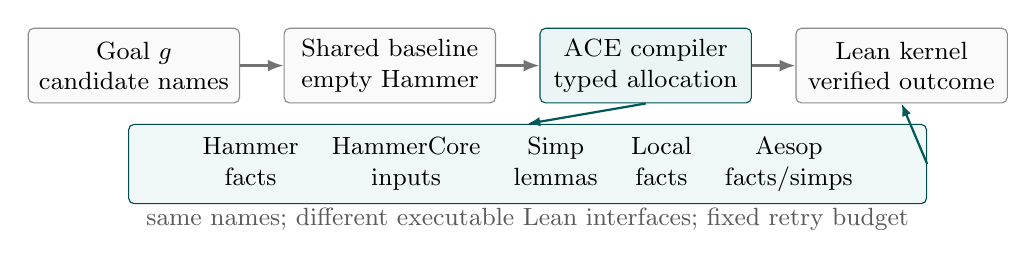
\begin{tikzpicture}[
font=\small,
stage/.style={draw=black!45, rounded corners=2pt, fill=black!2, align=center,
  minimum height=2.7em, text width=2.45cm},
routebar/.style={draw=teal!60!black, rounded corners=2pt, fill=teal!6, align=center,
  minimum height=2.35em, text width=9.9cm},
arrow/.style={-{Latex[length=2mm]}, thick, black!55},
taparrow/.style={-{Latex[length=1.6mm]}, thick, teal!70!black}
]
\node[stage] (goal) at (0,0) {Goal $g$\\candidate names};
\node[stage] (empty) at (3.25,0) {Shared baseline\\empty Hammer};
\node[stage, fill=teal!8, draw=teal!65!black] (alloc) at (6.5,0) {\tap{} compiler\\typed allocation};
\node[stage] (lean) at (9.75,0) {Lean kernel\\verified outcome};
\draw[arrow] (goal) -- (empty);
\draw[arrow] (empty) -- (alloc);
\draw[arrow] (alloc) -- (lean);

\node[routebar] (routes) at (5.0,-1.25)
  {\begin{tabular}{ccccc}
  Hammer & HammerCore & Simp & Local & Aesop\\
  facts & inputs & lemmas & facts & facts/simps
  \end{tabular}};
\draw[taparrow] (alloc.south) -- (routes.north);
\draw[taparrow] (routes.east) -- (lean.south);
\node[align=center, text=black!65] at (5.0,-1.95)
  {same names; different executable Lean interfaces; fixed retry budget};
\end{tikzpicture}
\vspace{-0.9em}
\caption{\tap{} evaluates action-conditional evidence allocation under a fixed retry budget. Selected names are compiled into typed Lean interfaces, and each routed action is checked by the Lean kernel.}
\label{fig:pipeline}
\end{figure}

\subsection{Typed Evidence Programs}

The allocator is built from action families that consume selected names differently. Hammer actions pass names as ordinary premises; HammerCore actions expose a smaller internal proof-search interface; simplification actions use selected names as rewrite/simp lemmas; local elimination uses names as local facts; Aesop actions can add names as fact rules, simp rules, or both. For each replayable theorem context, we materialize a patched pre-theorem Lean file for each action and classify the result by running Lean with a fixed timeout.

The fixed portfolio is chosen greedily on the training split and evaluated out of fold. Every policy receives the same first action, \texttt{hammer\_empty}, and then a retry budget $K$. This protocol makes the strongest control explicit: an adaptive policy is only useful if it beats or compresses the best fixed sequence of typed actions under the same Lean-call budget. In the current matrix, the train-fitted four-action portfolio after \texttt{hammer\_empty} combines Aesop, HammerCore, Hammer, and local-elimination actions.

This design also prevents a common misreading of the method. The fixed portfolio is not intended to prove that a hand-written order is optimal; it is the hard control that any learned action router must beat. Its near-oracle performance is therefore evidence that interface typing itself is a large effect, while the absence of an adaptive win is reported as a boundary rather than hidden as a negative result.

\subsection{Aesop Fact/Simp Exposure}

Aesop is the most important new interface in the verified matrix, so we isolate how selected names enter it. Given a ranked name list, we split available names into fact candidates and simp candidates, then instantiate Aesop in three exposure modes: facts-only, simps-only, and facts+simps. We also vary source pools: traced oracle-core names, retrieved-only names, and oracle-core plus retrieved names at budgets 8, 16, and 32. This gives a matched source/budget control: the goal and candidate source are fixed, while the channel assignment is removed, added, or widened.

The Aesop ablation is not a new oracle-improving action set; its role is explanatory. The original broad ablation suggested a strong facts+simps interaction, but exact matched controls give a more conservative readout. For the best current oracle-core plus retrieved source, joint exposure recovers the 38/230 Aesop result, yet identity exposure reaches 36/230, simps-only reaches 35/230, facts-only reaches 32/230, and joint-only over exact single-channel controls is only 2 goals. Retrieved-only joint exposure still reaches 34/230 and oracle-core-only reaches 35/230. The supported mechanism is therefore source/exposure/search sensitivity, not a clean causal claim that facts and simps are complementary in isolation.

\subsection{Why Typed Actions Should Help}

Let $Y_g(z;B)\in\{0,1\}$ denote the kernel-verified potential outcome for goal $g$ when typed assignment $z$ is checked under search budget $B$. The marginal intervention effect of exposing name $p$ through interface $\tau$ is
\[
\Delta_g(p,\tau\mid z,B)=Y_g(z+e_{p,\tau};B)-Y_g(z;B).
\]
This formulation is intentionally intervention-level rather than only a marginal retrieval score. It permits the same name to have positive effect in one interface and negative effect in another, allows facts and simp rules to interact through the current program $z$, and permits larger evidence sets to have negative marginal effect under bounded search. A typed action helps when the compiler finds assignments whose realized intervention effects are positive under the Lean backend's budget, not merely when a retriever ranks relevant names highly.

\section{Experiments}

\paragraph{Protocol.}
All main results are kernel-verified Lean checks in a Mathlib 4.30 + LeanHammer 4.30 pre-theorem replay harness. We first clean 490 traced-corpus goals and keep the 230 goals whose original tactic script replays before the theorem statement. We then run typed proof actions in Lean and count a success only when the patched file checks. To separate interface allocation from traced proof-core assistance, we repeat the budgeted compiler test with only retrieved candidates. Finally, we freeze the retrieved-only action subset and evaluate two disjoint 500-goal folds with zero overlap against the original 230-goal set; the folds contain 432 replayable goals in total. Trace-core and bridge experiments are retained in Appendix~\ref{tab:appendix-discovery-summary} as discovery evidence for bounded retries, not as the main proving metric.

\begin{table}[t]
\caption{Core verified evidence. ``Portfolio'' is the fixed typed retry sequence after the shared \texttt{hammer\_empty} call; the fresh-holdout row uses the frozen retrieved-only sequence and an oracle over the predeclared tested actions.}
\label{tab:core-results}
\centering
\small
\resizebox{\linewidth}{!}{
\begin{tabular}{lrrrrr}
\toprule
Setting & Empty & Best single & Portfolio & Oracle & Readout \\
\midrule
Mixed-source 230 & 29/230 & 38/230 & \best{57/230} OOF & 58/230 & typed actions create +20 oracle headroom \\
Retrieved-only 230 & 29/230 & 35/230 & \best{52/230} OOF & 52/230 & removes traced proof-core assistance \\
\rowcolor{teal!7}
Frozen fresh holdout & 30/432 & 54/432 & \best{67/432} & 68/432 & transfers beyond the discovery matrix \\
\bottomrule
\end{tabular}}
\end{table}

Table~\ref{tab:core-results} is the main empirical result. On the mixed-source 230-goal matrix, the best single typed action solves 38 goals, while the typed action oracle solves 58; a four-retry fixed portfolio reaches 57 out of fold. Removing traced proof-core names gives the retrieved-only anchor: the best standalone action solves 35/230, but the fixed typed portfolio reaches the 52/230 typed oracle. The frozen holdout check gives the same readout prospectively: on 432 replayable goals, the frozen K=4 sequence solves 67 goals, compared with 54 for the best singleton and 68 for the tested-action oracle. Thus the main effect is not a post-hoc fit to one matrix and not only an oracle-core artifact.

\begin{figure}[t]
\centering
\small
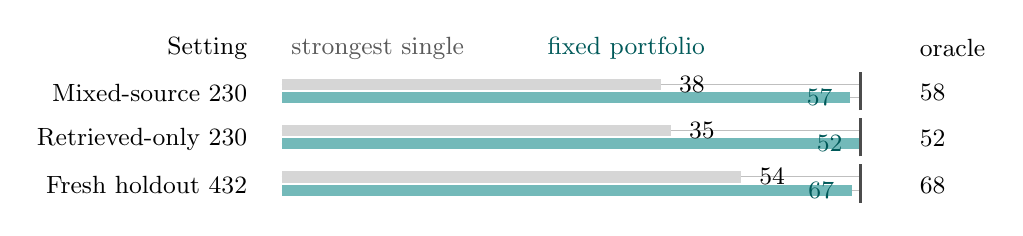
\begin{tikzpicture}[font=\small, x=0.105cm, y=0.42cm]
\node[anchor=east] at (0,4.85) {Setting};
\node[anchor=west, text=black!65] at (3,4.85) {strongest single};
\node[anchor=west, text=teal!70!black] at (34,4.85) {fixed portfolio};
\node[anchor=west] at (79,4.85) {oracle};

\foreach \label/\ys/\yp/\single/\port/\snum/\pnum/\onum in {
Mixed-source 230/3.75/3.35/45.9/68.8/38/57/58,
Retrieved-only 230/2.35/1.95/47.1/70.0/35/52/52,
Fresh holdout 432/0.95/0.55/55.6/69.0/54/67/68} {
  \node[anchor=east, align=right] at (0,\ys-0.25) {\label};
  \draw[black!25, line width=0.35pt] (3,\ys) -- (73,\ys);
  \draw[black!25, line width=0.35pt] (3,\yp) -- (73,\yp);
  \fill[black!16] (3,\ys-0.17) rectangle ++(\single,0.34);
  \fill[teal!55] (3,\yp-0.17) rectangle ++(\port,0.34);
  \draw[black!70, line width=0.8pt] (73,\yp-0.38) -- (73,\ys+0.38);
  \node[anchor=west] at (3+\single+1,\ys) {\snum};
  \node[anchor=east, text=teal!70!black] at (3+\port-1,\yp) {\pnum};
  \node[anchor=west] at (79,\ys-0.25) {\onum};
}
\end{tikzpicture}
\vspace{-0.9em}
\caption{Result ladder. Bars are normalized within each setting by the tested-action oracle. Across the mechanism matrix, deployability anchor, and frozen holdout, the fixed typed portfolio recovers most tested oracle headroom rather than merely improving on a weak singleton baseline.}
\label{fig:result-ladder}
\end{figure}

\begin{table}[t]
\caption{Budget path after the shared \texttt{hammer\_empty} call. The same typed-portfolio story holds in the mixed-source matrix, the retrieved-only anchor, and the frozen holdout.}
\label{tab:budget-path}
\centering
\small
\begin{tabular}{lrrrrr}
\toprule
Setting & K=1 & K=2 & K=3 & K=4 & Oracle \\
\midrule
Mixed-source 230 & 49/230 & 55/230 & 55/230 & \best{57/230} & 58/230 \\
Retrieved-only 230 & 47/230 & 50/230 & \best{52/230} & \best{52/230} & 52/230 \\
\rowcolor{teal!7}
Frozen holdout 432 & 56/432 & 58/432 & \best{67/432} & \best{67/432} & 68/432 \\
\bottomrule
\end{tabular}
\end{table}

Table~\ref{tab:budget-path} shows why the fixed sequence is a strong control rather than a weak baseline. In all three settings, the portfolio approaches the tested oracle quickly. On the retrieved-only anchor, K=3 already reaches the oracle. On the frozen holdout, K=3 and K=4 recover 67/68 tested-action opportunities, and the strict after-\texttt{hammer\_empty} coverage is 37/38. The remaining one-goal gap is useful because it shows that the frozen policy is not evaluated against a trivial oracle.

\begin{table}[t]
\caption{Fresh-holdout fold details. The action subset and order are frozen before evaluation; the two folds have zero overlap with the original 230-goal matrix.}
\label{tab:fresh-folds}
\centering
\small
\begin{tabular}{lrrrrrr}
\toprule
Fold & Replayable & Empty & Best single & K=3 & K=4 & Oracle \\
\midrule
Fold 0 & 208 & 16 & 23 & \best{28} & \best{28} & 28 \\
Fold 1 & 224 & 14 & 31 & 39 & 39 & \best{40} \\
\rowcolor{teal!7}
Combined & 432 & 30 & 54 & \best{67} & \best{67} & 68 \\
\bottomrule
\end{tabular}
\end{table}

Table~\ref{tab:fresh-folds} is the prospective check that matters most for presentation. The fold-level numbers are not identical, but both move in the same direction: the frozen typed sequence beats the strongest singleton, and the combined result is within one goal of the tested-action oracle. This is the main reason the paper can present fixed typed diversity as a real compiler effect rather than a training-set artifact.

\begin{table}[t]
\caption{Homogeneous K=4 controls under the same outer Lean-call budget on the mixed-source 230-goal matrix. Typed diversity beats repeated use of one proof-action family.}
\label{tab:family-controls}
\centering
\small
\begin{tabular}{lrr}
\toprule
Portfolio family & OOF K=4 & Strict goals \\
\midrule
\rowcolor{teal!7}
Full typed grid & \best{57/230} & \best{28/29} \\
Aesop-only & 49/230 & 20/29 \\
HammerCore-only & 41/230 & 12/29 \\
Simplification-only & 41/230 & 12/29 \\
Local-elimination-only & 34/230 & 5/29 \\
Hammer-only & 32/230 & 3/29 \\
Raw arithmetic/normalization & 29/230 & 0/29 \\
\bottomrule
\end{tabular}
\end{table}

Table~\ref{tab:family-controls} rules out a simple ``more retries'' explanation. Four Aesop retries are useful but remain eight goals behind the typed portfolio; HammerCore-only and simplification-only controls are much weaker; and Hammer-only barely improves over empty Hammer. The portfolio is strong because it crosses proof interfaces.

\begin{table}[t]
\caption{Learned allocator gate on the mixed-source 230-goal matrix. Learned routers match the fixed control at high budgets but do not beat or compress it.}
\label{tab:learned-gate}
\centering
\small
\begin{tabular}{rrrrr}
\toprule
K & Fixed OOF & Pure logreg & Residual logreg & Residual CNB \\
\midrule
1 & \best{49/230} & 41/230 & 41/230 & 38/230 \\
2 & \best{55/230} & 41/230 & \best{55/230} & 52/230 \\
3 & 55/230 & 44/230 & \best{56/230} & 55/230 \\
4 & \best{57/230} & 47/230 & \best{57/230} & \best{57/230} \\
\bottomrule
\end{tabular}
\end{table}

Table~\ref{tab:learned-gate} turns a negative result into a boundary on the claim. The learned gates see goal text, first-failure status, and typed fact/simp pool features, but they do not surpass the fixed typed control. This prevents an overclaim about adaptive routing and strengthens the paper's simpler message: the immediate missing layer after retrieval is typed compilation.

\begin{table}[t]
\caption{Exact Aesop source/channel controls. Joint exposure is best, but the matched controls support source/interface sensitivity rather than a large pure facts-versus-simps complementarity.}
\label{tab:aesop-controls}
\centering
\footnotesize
\begin{tabular}{lrr}
\toprule
Aesop control & Verified goals & Readout \\
\midrule
\texttt{empty} Aesop & 29/230 & default baseline \\
\texttt{retrieved-only}, joint & 34/230 & non-oracle source helps \\
\texttt{oracle-core-only}, joint & 35/230 & oracle source alone is similar \\
\rowcolor{teal!7}
\texttt{oracle-core+retrieved}, joint & \best{38/230} & best Aesop row \\
\texttt{oracle-core+retrieved}, identity & 36/230 & identity explains much of the lift \\
\texttt{oracle-core+retrieved}, simps-only & 35/230 & simp exposure is strong \\
\texttt{oracle-core+retrieved}, facts-only & 32/230 & fact exposure is weaker \\
\bottomrule
\end{tabular}
\end{table}

Table~\ref{tab:aesop-controls} keeps the mechanism claim calibrated. Aesop is an important interface, and joint exposure is the best Aesop row, but the gap over identity and simps-only controls is modest. This is why the paper's main claim is typed evidence allocation across interfaces, not a specialized claim that Aesop facts and simps form a large isolated complementarity.

\begin{table}[t]
\caption{Focused boundary checks. These controls rule out the main shortcuts while keeping the paper's claim narrow: the supported mechanism is typed interface allocation, not a learned-router or pure Aesop-channel claim.}
\label{tab:boundary}
\centering
\footnotesize
\resizebox{\linewidth}{!}{
\begin{tabular}{L{0.25\linewidth}L{0.38\linewidth}L{0.29\linewidth}}
\toprule
Question & Control result & Readout \\
\midrule
Is this just more calls to one backend? & Full typed K=4: 57/230; Aesop-only: 49/230; HammerCore/simp-only: 41/230; Hammer-only: 32/230. & Interface diversity matters. \\
Is learned routing the contribution? & Best logistic/ComplementNB gates match but do not beat fixed K=4: 57/230. & Fixed portfolio is the hard control. \\
Is Aesop facts+simps the whole story? & Joint oracle-core+retrieved: 38/230; identity: 36/230; simps-only: 35/230; facts-only: 32/230. & Source/interface sensitivity, not a large pure complementarity. \\
Does syntactic cleanup explain the gains? & Strict-filtered oracle: 4/230; combined oracle remains 58/230. & Cleanup alone is not the mechanism. \\
What is the call/time cost? & \texttt{hammer\_empty}: 29/230 at 1.00 calls, 8.31s; train-fitted K=4: 58/230 at 4.18 calls, 40.07s. & Main comparisons are matched by Lean calls; wallclock is transparent. \\
\bottomrule
\end{tabular}}
\end{table}

Table~\ref{tab:boundary} explains why we present \tap{} as a typed evidence compiler rather than as a generic portfolio or adaptive-router method. Repeating one family is weaker than mixing interfaces; learned routers do not yet compress the fixed control; Aesop exposure is useful but not a standalone explanation; and broad filtering does not recover the effect. These negative and diagnostic results are useful because they make the supported claim sharper: after a retriever proposes names, Lean still needs a typed decision about how those names enter proof search.

\section{Theory and Analysis}

\begin{proposition}[A scalar premise score cannot represent typed intervention value]
Let $Y_g(z;B)\in\{0,1\}$ be the kernel-verified outcome for goal $g$ under typed evidence assignment $z$ and search budget $B$. If there exist a name $p$ and two interfaces $\tau_1,\tau_2$ such that
\[
Y_g(z+e_{p,\tau_1};B)\ne Y_g(z+e_{p,\tau_2};B),
\]
then no interface-agnostic premise score for $p$ can represent the full intervention effect of exposing $p$ to Lean.
\end{proposition}

\noindent\textbf{Sketch.}
The intervention $e_{p,\tau}$ changes both the syntax sent to Lean and the backend search process that consumes the name. If two interface assignments yield different verified outcomes under the same goal and budget, a premise ranking over $p$ alone has discarded information needed to choose the successful action. This is the formal reason for compiling selected evidence into typed proof actions rather than treating retrieval as the final decision. Table~\ref{tab:core-results} gives the empirical version: the best single action is far below the typed oracle, while a small typed portfolio recovers nearly all tested headroom.

\begin{proposition}[Premise coverage is not monotonic in premise budget]
There can exist premise sets $P_1\subset P_2$ such that $P_1$ covers enough useful premises for the backend to succeed under budget $B$, while $P_2$ contains the same useful premises but causes timeout or reconstruction failure under the same budget.
\end{proposition}

\noindent\textbf{Sketch.}
Adding premises preserves proof-core coverage but can increase branching, generated clauses, simplification search, or reconstruction ambiguity. Under fixed time/search budget, the prover may fail on the larger set even though the smaller set contains the same proof-relevant lemmas. The boundary checks in Table~\ref{tab:boundary} are consistent with this view: broad Aesop insertion and strict syntactic filtering do not explain the gains, while typed diversity does.

\section{Scope and Deployment Notes}

The experiments are designed as a proof-action intervention study rather than a leaderboard entry. The main matrix uses 230 replayable pre-theorem Mathlib contexts, and the frozen holdout adds 432 replayable retrieved-only contexts with no overlap against the discovery set. This setup avoids target-theorem leakage and makes each reported success a kernel-checked Lean result. A full external deployment would naturally combine \tap{} with stronger global retrievers such as LeanSearch-style systems; our retrieved-only rows study the downstream compiler once such candidates have been proposed.

The current strongest policy is intentionally simple: a fixed typed portfolio. This is a useful property for the present claim because it shows that much of the headroom comes from interface typing itself, before more complex adaptive routing is needed. Learned routers, trace-core controllers, wallclock frontiers, and bridge diagnostics are therefore reported as supporting analyses rather than as the paper's central promise.

\section{Discussion}

\paragraph{What changes for Lean premise systems?}
The practical implication is that a premise selector should not hand a prover only an ordered list of names. It should hand off a typed evidence program: which names are ordinary Hammer facts, which are HammerCore inputs, which are simplification lemmas, which are elimination facts, and which are Aesop fact or simp rules. This is a small interface change but a different abstraction boundary. Retrieval remains responsible for proposing useful names; the compiler layer decides how those names become executable proof actions.

\paragraph{Why the fixed portfolio is informative.}
The fixed portfolio is not presented as an optimal hand-written strategy. It is the strongest failure-agnostic control we found under the same outer retry budget. Its near-oracle behavior is exactly what makes the result interesting: much of the current headroom is recovered by crossing typed interfaces at all, before asking a learned router to decide per goal. This also sets a higher bar for future adaptive methods. A router should not be compared only to empty Hammer or to a single tactic; it should beat a compact typed portfolio.

\begin{table}[t]
\caption{How each evidence block supports the main claim. The rows are ordered by the role they play in the argument, not by when the experiments were run.}
\label{tab:argument-map}
\centering
\small
\resizebox{\linewidth}{!}{
\begin{tabular}{L{0.24\linewidth}L{0.32\linewidth}L{0.34\linewidth}}
\toprule
Role in the argument & Evidence used in the main text & What it rules out \\
\midrule
Interface effect exists & 58/230 typed oracle vs 38/230 best single; 57/230 fixed OOF. & The result is not just one strong tactic. \\
Not trace-core leakage & Retrieved-only portfolio reaches 52/230 vs 35/230 best single. & The effect does not require traced proof-core names. \\
Not post-hoc overfit & Frozen holdout reaches 67/432 vs 54/432 best singleton. & The portfolio is not only fit to the discovery matrix. \\
Not repeated backend calls & Homogeneous K=4 controls are below full typed K=4. & The gain comes from typed diversity. \\
Not an adaptive-router claim & Learned gates match but do not beat fixed K=4. & The paper's contribution is the typed compiler layer. \\
\bottomrule
\end{tabular}}
\end{table}

\paragraph{A compiler checklist for future systems.}
The experiments suggest a simple reporting and implementation checklist for retrieval-augmented Lean provers. First, report the candidate source separately from the proof-action interface; otherwise a retrieval failure and an interface-compilation failure are indistinguishable. Second, include a fixed typed portfolio as a static control before claiming that an adaptive router is useful. Third, report a retrieved-only version of the compiler test when traced proof-core names are available during development. Fourth, report whether extra names are helping the backend or merely increasing search and reconstruction cost.

\begin{table}[t]
\caption{Practical checklist induced by the experiments. Each row corresponds to a common ambiguity in retrieval-augmented proving.}
\label{tab:compiler-checklist}
\centering
\small
\resizebox{\linewidth}{!}{
\begin{tabular}{L{0.25\linewidth}L{0.31\linewidth}L{0.34\linewidth}}
\toprule
Question for a Lean prover & Recommended measurement & Why it matters \\
\midrule
Did retrieval or interface compilation fail? & Separate candidate source, typed action, and verified outcome. & A good name list can still fail under the wrong interface. \\
Is a learned router truly useful? & Compare against the best fixed typed portfolio at the same K. & Empty Hammer and single actions are too weak as controls. \\
Does the effect depend on proof traces? & Run a retrieved-only compiler anchor. & This separates deployable candidate use from oracle-core assistance. \\
Does more evidence help or hurt? & Report strict goals, homogeneous families, and wallclock. & Premise coverage and proof-search tractability can diverge. \\
\bottomrule
\end{tabular}}
\end{table}

\paragraph{Why this checklist is conservative.}
The checklist does not require a new benchmark or a new global retriever. It can be applied to any retrieval source that proposes Lean names: a learned retriever, a lexical retriever, a search-based retriever, or a human-provided candidate list. That makes \tap{} a modular compiler layer. Its job is not to decide which names are globally relevant; its job is to make a selected candidate set executable under the proof interfaces that Lean actually provides.

\paragraph{Why this is not only a benchmark result.}
The main result is an intervention on the proof interface, not a new leaderboard score. The same candidate source can produce different verified outcomes depending on how names enter Lean. This creates a reusable diagnostic for future prover work: when a retriever appears weak, one should ask whether the missing step is retrieval quality or evidence compilation. Conversely, when a large premise set hurts, the remedy may be a different typed action rather than another reranking pass over the same untyped list.

\paragraph{How to read the remaining failures.}
The unsolved goals are also informative because the intervention protocol localizes them. A miss after every single typed action points to candidate quality; a miss after the full portfolio points to missing proof actions, longer reasoning chains, or backend search limits. Thus the oracle, homogeneous, strict-goal, and retrieved-only controls turn raw failures into a map of where the prover stack should improve next.

\paragraph{What a stronger next system should do.}
The natural next step is to learn an allocator that beats the fixed typed portfolio while preserving the same accounting discipline: same first attempt, same retry budget, same verified-outcome metric, and the same strong static controls. The present experiments identify where the oracle headroom is, show that a simple typed sequence captures most of it, and separate the compiler effect from both traced proof-core assistance and post-hoc portfolio fitting.

\section{Conclusion}

This paper argues that Lean premise selection is incomplete without action-conditional evidence allocation. \tap{} implements this view as a typed evidence compiler over Hammer, HammerCore, simplification, local-elimination, and Aesop interfaces. In the mixed-source 230-goal matrix, the typed action grid reaches 58/230 verified proofs versus 38/230 for the best single action, and a four-retry fixed typed control recovers 57/230 out of fold. In the retrieved-only anchor, the same compiler view reaches 52/230 with a fixed portfolio, compared with 29/230 for empty Hammer and 35/230 for the best standalone action. In two frozen fresh-holdout folds, the predeclared K=4 portfolio solves 67/432 replayable goals versus 54/432 for the best singleton and 68/432 for the tested-action oracle. The exact Aesop controls make the mechanism more precise: source and interface assignment matter, but a large pure facts-versus-simps complementarity is not supported. The result is a narrow but concrete lesson for Lean provers: retrieval should hand off not just a list of names, but a typed evidence program that tells Lean how those names should enter proof search. More broadly, the evaluated unit should be a candidate name together with its consuming interface, because the same evidence can help, fail, or hurt under different proof actions.

\newpage
\bibliography{references}
\bibliographystyle{iclr2026_conference}

\appendix

\section{Additional Experimental Details}

\subsection{Canonical Output Sources}

All numbers in the main tables are copied from canonical JSON or Markdown outputs in the project directory:
\begingroup
\footnotesize
\sloppy
\begin{itemize}[leftmargin=*,itemsep=1pt]
\item Verified typed action grid: \url{outputs/mathlib430_pretheorem_action_matrix_scaled230_aesop_ablation_merged.md}.
\item Budgeted typed portfolio: \url{outputs/mathlib430_budgeted_action_policy_scaled230_aesop_ablation.md}.
\item Typed allocator gate: \url{outputs/mathlib430_typed_allocator_gate_scaled230_aesop_ablation.md}.
\item Retrieved-only anchor summary: \url{analysis/mathlib430_retrieved_only_anchor_summary.md}.
\item Retrieved-only anchor matrix: \url{outputs/mathlib430_pretheorem_action_matrix_scaled230_retrieved_only_anchor_merged.md}.
\item Retrieved-only fixed stability: \url{outputs/mathlib430_fixed_portfolio_stability_scaled230_retrieved_only_anchor.md}.
\item Frozen fresh-holdout summary: \url{analysis/mathlib430_fresh_holdout_summary.md}.
\item Fresh-holdout fold summaries: \url{analysis/mathlib430_fresh_holdout_fold0_summary.md} and \url{analysis/mathlib430_fresh_holdout_fold1_summary.md}.
\item Fresh-holdout merged action outputs: \url{outputs/mathlib430_fresh_holdout_fold0_frozen_actions_merged.md} and \url{outputs/mathlib430_fresh_holdout_fold1_frozen_actions_merged.md}.
\item Exact Aesop source/channel controls: \url{analysis/mathlib430_aesop_exact_controls_summary.md}.
\item Initial broad Aesop fact/simp ablation: \url{analysis/mathlib430_aesop_ablation_scaled230.md}.
\item Initial Aesop counterfactual channel control: \url{analysis/mathlib430_aesop_counterfactual_controls.md}.
\item Evidence-contract audit and homogeneous controls: \url{analysis/mathlib430_evidence_contract_audit.md}.
\item Strict interface filtering boundary: \url{analysis/mathlib430_e1_strict_interface_filtering.md}.
\item Strict interface taxonomy: \url{analysis/mathlib430_strict_action_taxonomy_scaled230_aesop_ablation.md}.
\item Local trace-core: \url{outputs/phase1_mathlib_trace_core_2000_feature_ablation_a40.json}.
\item Phase 1 bridge: \url{outputs/phase1_reconstruction_bridge_report_100.md}.
\item Timeout stress: \url{outputs/phase2_timeout_stress_2000_a40.json}.
\item Imported-core heldout: \url{outputs/phase3_second_stage_controller_eval_500_a40.json} plus final guardrail deltas.
\item Split stability: \url{outputs/phase3_split_stability_summary_4x500.md}.
\item Imported bridge report: \url{outputs/phase3_bridge_report_200.md}.
\item Imported bridge taxonomy: \url{outputs/phase3_bridge_failure_taxonomy_200.md}.
\item Imported bridge inspection: \url{outputs/phase3_bridge_negative_case_inspection_200.md}.
\end{itemize}
\endgroup

\subsection{Trace-Core Discovery Summary}

\begin{table}[H]
\caption{Representative trace-core discovery results that motivated the verified typed-action protocol. These rows are not the main proving metric; they explain the design pressure for bounded retries, non-monotonic premise budgets, and bridge checks.}
\label{tab:appendix-discovery-summary}
\centering
\footnotesize
\begin{tabular}{@{}L{0.28\linewidth}L{0.34\linewidth}L{0.28\linewidth}@{}}
\toprule
Discovery question & Strongest useful result & Readout for current paper \\
\midrule
Can failure feedback improve local premise recovery? & Local trace-core \far{} reaches 95.7\% trace success and 72.0\% bridge verified success; blind top-$k$ expansion reaches 91.5\% trace and 43.0\% bridge. & Failure events can change which evidence is useful, but bridge verification is stricter than trace-core recovery. \\
Can adding more premises hurt? & Timeout-conditioned shrink reaches 69.3\% success with 23.5\% timeout rate, while equal-budget top-$k$ falls to 43.8\% with 56.2\% timeouts. & Premise coverage is not monotonic under bounded search, motivating typed budgets instead of broad insertion. \\
Do local heuristics solve global imported premises? & Imported-core lexical/BM25 stress stays near 12\% success before learned retrieval. & Local feature control is insufficient for global retrieval; the verified paper should not claim full retriever replacement. \\
Does learned imported retrieval survive bridge checks? & Final-base8 averages 92.9\% across four splits and reaches 53.5\% imported bridge verified success versus 44.5\% for learned+base fallback. & Bridge evidence supports the premise-recovery story but remains separate from open-ended proof generation. \\
\bottomrule
\end{tabular}
\end{table}

\subsection{Feature-Group Ablation}

\begin{table}[H]
\caption{Feature-group ablation on 2k local trace-core goals. Static visible-feature reranking is weaker than blind expansion; failure-conditioned feature use is the important step.}
\label{tab:appendix-feature}
\centering
\small
\begin{tabular}{lrrr}
\toprule
Method & Success & FFR & Avg prem. \\
\midrule
\texttt{topk\_expansion} & 91.5\% & 79.9\% & 46.9 \\
\texttt{visible\_feature\_name\_rerank} & 85.3\% & 0.0\% & 42.9 \\
\texttt{visible\_feature\_statement\_rerank} & 77.6\% & 0.0\% & 42.9 \\
\texttt{visible\_feature\_decl\_rerank} & 78.3\% & 0.0\% & 42.9 \\
\texttt{visible\_feature\_rerank} & 86.5\% & 0.0\% & 42.9 \\
\texttt{rule\_far\_no\_core\_decl\_features} & 92.6\% & 82.4\% & 46.2 \\
\texttt{rule\_far\_no\_core\_statement\_features} & 92.8\% & 82.9\% & 46.4 \\
\texttt{rule\_far\_no\_core\_name\_features} & 95.0\% & 88.1\% & 45.4 \\
\texttt{rule\_far\_no\_core\_tags} & \best{95.7\%} & \best{89.7\%} & 45.1 \\
\bottomrule
\end{tabular}
\end{table}

\subsection{Imported-Core Stress Before Learned Retrieval}

\begin{table}[H]
\caption{Initial imported-core stress test on 2k goals. This table is a diagnostic negative result: local and lexical signals are insufficient for global imported-premise recovery.}
\label{tab:appendix-global-stress}
\centering
\small
\begin{tabular}{lrrr}
\toprule
Method & Success & FFR & Avg prem. \\
\midrule
\texttt{one\_shot} & 1.1\% & 0.0\% & 32.0 \\
\texttt{same\_file\_prior\_rerank} & 2.1\% & 0.0\% & 56.0 \\
\texttt{visible\_feature\_rerank} & 2.4\% & 0.0\% & 56.0 \\
\texttt{bm25\_rerank} & 7.0\% & 0.0\% & 56.0 \\
\texttt{leansearch\_iterative} & 11.9\% & 8.3\% & 91.9 \\
\texttt{bm25\_expansion} & 11.9\% & 8.3\% & 92.2 \\
\texttt{rule\_far\_bm25} & \best{12.2\%} & \best{8.7\%} & 92.2 \\
\texttt{rule\_far\_full} {\small (oracle ref.)} & 55.7\% & 55.2\% & 86.6 \\
\bottomrule
\end{tabular}
\end{table}

\subsection{Bridge Failure Taxonomy}

The 200-goal imported bridge verifies 124/200 original traced tactic scripts. The primary replay failures are 30 unknown-identifier errors, 13 other Lean errors, 8 typeclass failures, 7 unsolved-goal failures, 6 \texttt{simp} no-progress failures, 5 tactic failures, 5 type mismatches, and 2 sorry-context failures. At the policy level, final-base8 has 17 replay-verified trace misses, compared with 19 for the original second-stage controller, 35 for learned+base fallback, and 47 for learned expansion. Negative-case inspection finds 0/17 candidate-pool misses, 2 fallback-selected core drops, 3 expansion-selected core drops, and 15 failure-conditioned rank misses. This supports the limitation that remaining headroom is ranking and calibration, not candidate generation.

\subsection{Guardrail and Expert-Mixing Ablations}

The final base8 guardrail was selected because broader heuristics were negative. Hard base guardrails reduce bridge trace-core success from 72.0\% to 63.0\% or 60.0\%. Soft base-score mixing is inert at low mixing weights and harmful at high weights. Imported-failure multi-expert routing drops bridge trace-core success to 62.0\%. A larger final expert guardrail also underperforms final-base8 on the original split, fold0, and bridge subset. These results justify stopping hand-written expert-mix tuning and treating calibrated expert gating as future work.

\section{Claim-Evidence Self-Review}

\begin{table}[H]
\caption{End-of-draft self-review. Claims in the abstract and introduction are aligned to reported evidence; unsupported stronger claims are explicitly avoided.}
\label{tab:self-review}
\centering
\footnotesize
\begin{tabular}{@{}L{0.17\linewidth}L{0.46\linewidth}L{0.29\linewidth}@{}}
\toprule
Dimension & Current answer & Residual risk \\
\midrule
Contribution & Action-conditional evidence allocation is formulated as distinct from premise ranking, with frozen holdout and Aesop controls separating the core claim from mechanism diagnostics. & A fixed portfolio can look simple unless the typed-interface intervention remains central. \\
Writing clarity & Main text now leads with three verified layers: mixed-source matrix, retrieved-only anchor, and frozen fresh holdout; trace-core is kept as discovery evidence. & Method names are long; final draft may need shorter aliases. \\
Experiments & Results cover verified replayable Mathlib actions, budgeted allocators, retrieved-only compilation, frozen fresh-holdout folds, Aesop counterfactuals, trace-core discovery, and replay bridges. & Full action grid is still 230/490; holdout is retrieved-only and not a population-scale benchmark. \\
Evaluation & Kernel-verified action success, oracle headroom, fixed-budget policy, holdout transfer, and interface ablations are reported. & Full open-ended theorem proving and official retriever comparison are out of scope. \\
Soundness & Negative gates show broad insertion, strict syntactic filtering, and learned adaptive allocation are not enough. & Learned allocation does not yet beat the fixed typed control. \\
\bottomrule
\end{tabular}
\end{table}

\end{document}
